\section{Ход работы}
\subsection{Измерения}

1. Измерены константы установки:

\begin{itemize}
    \item $R = (114,1 \pm 0,5)$ мм,
    \item $r = \left(30,5 \pm 0,5\right)$ мм,
    \item $m = \left(1004,8 \pm 0,5\right)$ г,
    \item $z_0 = \left(220 \pm 1\right)$ см.
\end{itemize}

2. Измерены некоторые велчины тел, момент инерции которых стоит
измерить:
\begin{itemize}
    \item Диск: масса $m_\text{диск} = \left(587,6 \pm 0,1\right)$ г, диаметр $d_\text{диск} = (170,5 \pm 1)$ мм
    \item Кольцо: масса $m_\text{кольцо} = \left(581,3 \pm 0,1\right)$ г, внешний диаметр $d_\text{внеш} = \left(167,0 \pm 0,1\right)$ мм, внутренний диаметр $d_\text{внутр} = \left(156,6 \pm 0,1\right)$ мм
    \item Полукруг №1: масса $m_1 = \left(526,6 \pm 0,1\right)$ г, диаметр $d_1 = \left(80,0 \pm 0,1\right)$ мм
    \item Полукруг №2: масса $m_2 = \left(526,1 \pm 0,1\right)$ г, диаметр $d_2 = \left(79,8 \pm 0,1\right)$ мм
\end{itemize}

3. Измерены периоды колебаний на трифилярном подвесе
(погрешность измерения времени $\Delta t = 10^{-3}$ с):
\begin{center}
\begin{tabular}{|c|c|c|c|c|c|c|}
    \hline
    \multirow{2}{*}{Название} & \multicolumn{2}{c|}{Кол-во колебаний} & \multicolumn{2}{c|}{Время, с} & \multicolumn{2}{c|}{Период колбаний}\\
    \cline{2-7}
    & Изм. 1& Изм. 2& Изм. 1& Изм. 2& Изм. 1& Изм. 2\\
    \hline
    Диск & 11& 10 & 43,597 & 40,146 & 3,963 & 4,015\\
    \hline
    Кольцо &12&10&51,368&42,685&4,281&4,269\\
    \hline
    2 полукруга&10&10&32,816&32,775&3,282&3,276\\
    \hline
    Кольцо и диск&10&10&40,134&41,036&4,013&4,104\\
    \hline
    Без груза&10&11&44,462&48,712&4,446&4,428\\
    \hline
\end{tabular}
\end{center}

\begin{figure}[H]
    \centering
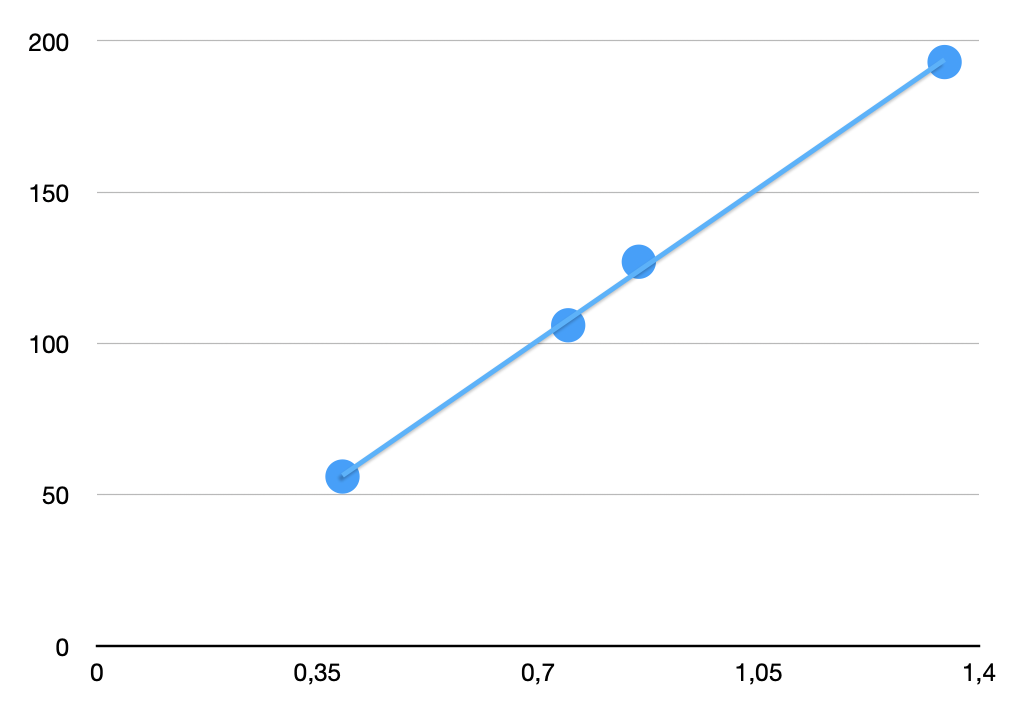
\includegraphics[width=0.4\linewidth,center]{p2.png}
    \caption{Расположение тел на платформе}
    \label{fig:my_label}
\end{figure}

4. Далее измерены для разных $h$ (рис. 2) периоды колебаний:
\begin{center}
\begin{tabular}{|c|c|c|c|}
    \hline
    $2h$, см & Кол-во колебаний & Время, с & Период, с\\
    \hline
    1 & 10 & 32.963 & 3.296 \\
\hline
   2 & 10 & 33.038 & 3.304 \\
\hline
   3 & 12 & 40.051 & 3.338 \\
\hline
   4 & 10 & 33.584 & 3.358 \\
\hline
   5 & 11 & 37.599 & 3.418 \\
\hline
   6 & 10 & 34.626 & 3.463 \\
\hline
   7 & 10 & 35.136 & 3.514 \\
\hline
   8 & 10 & 36.016 & 3.602 \\
\hline
   9 & 10 & 36.849 & 3.685 \\
\hline
   10 & 16 & 59.835 & 3.740 \\
\hline
   11 & 10 & 38.420 & 3.842 \\
\hline
   12 & 10 & 39.258 & 3.926 \\
\hline
   13 & 10 & 40.895 & 4.090 \\
\hline
   14 & 10 & 41.806 & 4.181 \\
\hline
   15 & 10 & 42.293 & 4.229 \\
\hline
   16 & 10 & 43.563 & 4.356 \\
\hline
   17 & 10 & 44.855 & 4.486 \\
\hline
   18 & 10 & 46.054 & 4.605 \\
\hline
   19 & 10 & 38.325 & 3.833 \\
\hline

\end{tabular}
\end{center}

\subsection{Обработка}

5. Расчитаем коэфициент k для подвеса из (9):
\begin{equation*}
    k = \frac{gRr}{4\pi^2z_0} = \left(393 \pm 7\right) \cdot 10^{-6} \text{ } \frac{\text{м}^2}{\text{с}^2}
\end{equation*}

6. Расчитаем моменты инерции для тел, участвующих в
эсперименте относительно центра масс по оси, перпендикулярной
плоскости тела (для тел используется адъитивность формула
$I_\text{тело} = k\left(m + m_\text{тeло}\right)T^2 - I$:
\begin{itemize}
    \item $I = \left(777 \pm 17\right) \cdot 10^{-5} \text{ кг} \cdot \text{м}^2$,
    \item $I_\text{диск} = (218 \pm 18) \cdot 10^{-5} \text{ кг} \cdot \text {м}^2$,
    \item $I_\text{кольцо} = \left(362 \pm 21\right) \cdot 10^{-5} \text{ кг} \cdot \text {м}^2$
    \item $I_\text{кольцо+диск} = \left(629 \pm 25\right) \cdot 10^{-5} \text{ кг} \cdot \text {м}^2$
    \item $I_\text{полукруги} = \left(92 \pm 15\right) \cdot 10^{-5} \text{ кг} \cdot \text {м}^2$
\end{itemize}

7. Далее построим зависимость $I\left(4h^2\right)$:

\begin{figure}[H]
    \centering
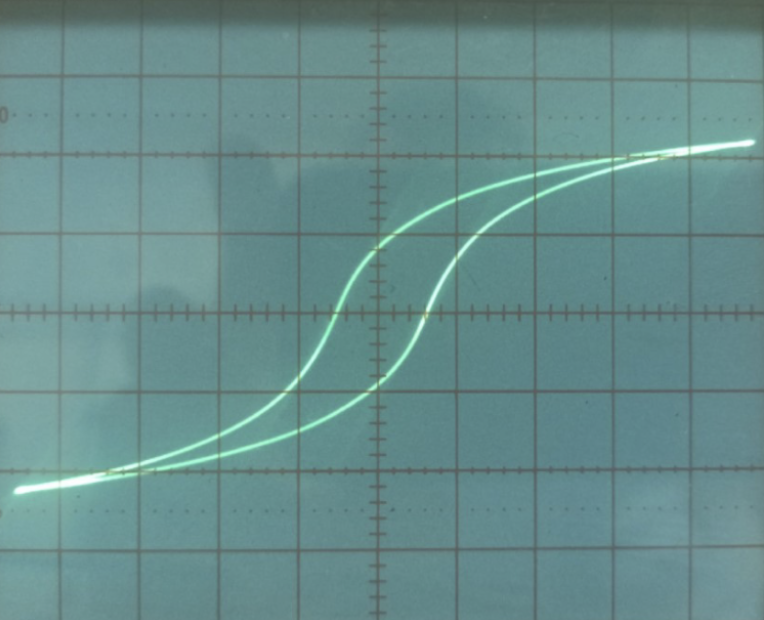
\includegraphics[width=0.75\linewidth,center]{p3.png}
    \label{fig:my_label}
\end{figure}

график зависимости имеет зависимость
$I = I\left(4h^2\right) = \left(871 + 3 \cdot 4h^2\right) \cdot 10^{-5} \text{ кг} \cdot \text {м}^2$.

8. Вычислим из этого момент инерции диска (масса считается
известной), используя теорему Гюйгенса-Штейнера:
\begin{equation*}
    I = \left(89 \pm 8\right) \cdot 10^{-5} \text{ кг} \cdot \text{м}^2
\end{equation*}

9. Посчитаем моменты инерции, используя формулу (1):
\begin{itemize}
    \item $I_\text{диск} = (2135 \pm 3) \cdot 10^{-6} \text{ кг} \cdot \text{м}^2$
    \item $I_\text{кольцо} = \left(3804 \pm 2\right) \cdot 10^{-6} \text{ кг} \cdot \text{м}^2$
    \item $I_\text{полукуги} = \left(842 \pm 2\right) \cdot 10^{-6} \text{ кг} \cdot \text{м}^2$
\end{itemize}
